\documentclass[10pt]{beamer}

% Packages
\usepackage[utf8]{inputenc}
\usepackage[T1]{fontenc}
\usepackage{amsmath, amssymb, amsthm}
\usepackage{graphicx}
\usepackage{booktabs}
\usepackage{hyperref}
\usepackage{tikz}
\usetikzlibrary{shapes,arrows,positioning}

% Theme settings
\usetheme{default}
\usecolortheme{default}
\usefonttheme{professionalfonts}

% Color definitions
\definecolor{ThemeBlue}{RGB}{0, 62, 116}
\definecolor{DarkGray}{RGB}{51, 51, 51}
\definecolor{LightGray}{RGB}{245, 245, 245}
\definecolor{AccentOrange}{RGB}{214, 96, 77}
\definecolor{AccentGreen}{RGB}{46, 139, 87}

% Apply colors
\setbeamercolor{frametitle}{fg=ThemeBlue, bg=white}
\setbeamercolor{title}{fg=ThemeBlue}
\setbeamercolor{structure}{fg=ThemeBlue}
\setbeamercolor{normal text}{fg=DarkGray}
\setbeamercolor{block title}{fg=white, bg=ThemeBlue}
\setbeamercolor{block body}{fg=DarkGray, bg=LightGray}
\setbeamercolor{itemize item}{fg=ThemeBlue}
\setbeamercolor{enumerate item}{fg=ThemeBlue}

% Remove navigation symbols
\setbeamertemplate{navigation symbols}{}

% Customize frame title
\setbeamertemplate{frametitle}{
  \vspace{0.5em}
  \insertframetitle
  \vspace{0.3em}
}

% Customize itemize
\setbeamertemplate{itemize items}[circle]
\setlength{\leftmargini}{1.5em}

% Footer
\setbeamertemplate{footline}{
  \leavevmode%
  \hbox{%
  \begin{beamercolorbox}[wd=.333333\paperwidth,ht=2.25ex,dp=1ex,left]{author in head/foot}%
    \hspace{1em}\usebeamerfont{author in head/foot}\insertshortauthor
  \end{beamercolorbox}%
  \begin{beamercolorbox}[wd=.333333\paperwidth,ht=2.25ex,dp=1ex,center]{title in head/foot}%
    \usebeamerfont{title in head/foot}\insertshorttitle
  \end{beamercolorbox}%
  \begin{beamercolorbox}[wd=.333333\paperwidth,ht=2.25ex,dp=1ex,right]{date in head/foot}%
    \usebeamerfont{date in head/foot}\insertshortdate{}\hspace*{2em}
    \insertframenumber{} / \inserttotalframenumber\hspace*{2ex} 
  \end{beamercolorbox}}%
  \vskip0pt%
}

% Commands
\newcommand{\highlight}[1]{\textcolor{AccentOrange}{\textbf{#1}}}
\newcommand{\good}[1]{\textcolor{AccentGreen}{#1}}
\newcommand{\bad}[1]{\textcolor{AccentOrange}{#1}}

% Mathematical operators
\DeclareMathOperator*{\argmin}{arg\,min}
\DeclareMathOperator{\E}{\mathbb{E}}
\DeclareMathOperator{\Var}{Var}

%----------------------------------------------------------------------------------------
\title{Big Data in Finance}
\subtitle{Week 1: Foundations of Machine Learning}
\author{Dr Daniele Bianchi}
\date{Spring 2026}
%----------------------------------------------------------------------------------------

\begin{document}

\AtBeginSection[]{
  \begin{frame}[plain]
    \vfill
    \begin{center}
      {\Large\color{ThemeBlue}\insertsection}
    \end{center}
    \vfill
  \end{frame}
}


\begin{frame}[plain]
  \titlepage
\end{frame}



\begin{frame}{Today's Agenda}
  \tableofcontents
\end{frame}

%----------------------------------------------------------------------------------------
\section{Introduction: What Are We Trying to Do?}
%----------------------------------------------------------------------------------------

\begin{frame}{The Core Question of This Module}
  \begin{center}
    \Large
    Can we make \highlight{better use} of data to improve \highlight{predictions} about financial outcomes?
  \end{center}
  
  \vspace{2em}
  \textbf{Examples we'll tackle in this course:}
  \begin{itemize}
    \item Which stocks will outperform next month and why?
    \item Will this borrower default on their loan and why?
  \end{itemize}
  
  \vspace{1em}
  \textbf{The challenge:} Financial markets are noisy, correlations and volatility change over time, and many claimed patterns do not hold up out-of-sample.
\end{frame}

\begin{frame}{A Concrete Example: Predicting Stock Returns}
  \textbf{Setup:} You're a portfolio manager trying to pick winning stocks
  
  \vspace{0.5em}
  \textbf{Data-Rich Environment}
  \begin{itemize}
    \item Company financials: earnings, book value, debt levels
    \item Market data: past returns, trading volume, volatility
    \item Valuation ratios: price-to-earnings, price-to-book
    \item Momentum: how has the stock performed recently?
  \end{itemize}
  
  \vspace{0.5em}
  \textbf{What Do You Want to Predict?}
  \begin{itemize}
    \item Next month's stock return (or just: will it beat the market?)
  \end{itemize}
  
  \vspace{0.5em}
  \textbf{The Machine Learning (ML) Approach:}
  \begin{enumerate}
    \item Collect historical data on stock characteristics and returns
    \item Learn the relationship between characteristics and subsequent returns
    \item Apply this relationship to make predictions as new data on characteristics arrive. 
  \end{enumerate}
\end{frame}

\begin{frame}{Learning from Data $\neq$ Fitting the Data}
\begin{center}
  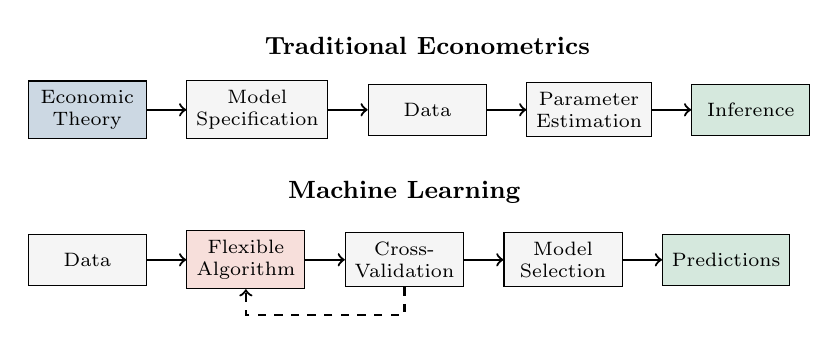
\begin{tikzpicture}[
    scale=1,
    transform shape,
    node distance=0.4cm and 0.5cm,
    box/.style={draw, rectangle, minimum width=1.5cm, minimum height=0.65cm, align=center, font=\scriptsize},
    arrow/.style={->, thick}
  ]
    % Econometrics approach
    \node[box, fill=ThemeBlue!20] (theory) {Economic\\Theory};
    \node[box, fill=LightGray, right=of theory] (model1) {Model\\Specification};
    \node[box, fill=LightGray, right=of model1] (data1) {Data};
    \node[box, fill=LightGray, right=of data1] (estimate) {Parameter\\Estimation};
    \node[box, fill=AccentGreen!20, right=of estimate] (inference) {Inference};
    
    \draw[arrow] (theory) -- (model1);
    \draw[arrow] (model1) -- (data1);
    \draw[arrow] (data1) -- (estimate);
    \draw[arrow] (estimate) -- (inference);
    
    \node[above=0.25cm of data1] {\small\textbf{Traditional Econometrics}};
    
    % ML approach
    \node[box, fill=LightGray, below=1.2cm of theory] (data2) {Data};
    \node[box, fill=AccentOrange!20, right=of data2] (algo) {Flexible\\Algorithm};
    \node[box, fill=LightGray, right=of algo] (validate) {Cross-\\Validation};
    \node[box, fill=LightGray, right=of validate] (select) {Model\\Selection};
    \node[box, fill=AccentGreen!20, right=of select] (predict) {Predictions};
    
    \draw[arrow] (data2) -- (algo);
    \draw[arrow] (algo) -- (validate);
    \draw[arrow] (validate) -- (select);
    \draw[arrow] (select) -- (predict);
    
    \draw[arrow, dashed] (validate.south) -- ++(0,-0.35) -| (algo.south);
    
    \node[above=0.25cm of validate] {\small\textbf{Machine Learning}};
  \end{tikzpicture}
\end{center}
  
%\vspace{0.3em}
%\small
\begin{center}
\begin{tabular}{lll}
\toprule
& \textbf{Econometrics} & \textbf{Machine Learning} \\
\midrule
Primary goal & Understand \emph{why} & Predict \emph{what} \\
%Key question & Does $X$ cause $Y$? & Does $X$ predict $Y$? \\
Model structure & Often theory-driven & Mostly data-driven \\
Variables & Few, interpretable & Many, algorithm selects \\
Focus & Statistical significance & Out-of-sample accuracy \\
\bottomrule
\end{tabular}
\end{center}

\vspace{0.5em}
\textbf{Punchline}: ML for prediction, econometrics for causal understanding. Good practitioners combine both as much as possible. 

% \begin{block}{They Are Complementary}
%   ML for prediction, econometrics for causal understanding. Good practitioners use both.
% \end{block}
\end{frame}



%----------------------------------------------------------------------------------------
\section{Problem Setup}
%----------------------------------------------------------------------------------------

\begin{frame}{Notation: Keeping It Simple}
  \textbf{Let's establish clear notation we will use throughout:}
  
  \vspace{0.5em}
  \begin{itemize}
    \item $x$ = \textbf{features} (the information we use to predict)
    \begin{itemize}
      \item For a single observation: $x = (x_1, x_2, \ldots, x_p)$
      \item Example: size, value ratio, momentum, profitability
    \end{itemize}
    \vspace{0.3em}
    \item $y$ = \textbf{target} (what we're trying to predict)
    \begin{itemize}
      \item Example: next month's return
    \end{itemize}
    \vspace{0.3em}
    \item $n$ = number of observations (e.g., stock-months)
    \item $p$ = number of features
  \end{itemize}
  
  \vspace{1em}
  \textbf{Our data structure:} We observe $n$ examples:
  \[
  (x^{(1)}, y^{(1)}), \; (x^{(2)}, y^{(2)}), \; \ldots, \; (x^{(n)}, y^{(n)})
  \]
  
  \vspace{0.3em}
  Each $x^{(i)} = (x_1^{(i)}, \ldots, x_p^{(i)})$ is a vector of $p$ features; each $y^{(i)}$ is the outcome.
\end{frame}


\begin{frame}{The Goal: Learn a Prediction Rule}
  \textbf{We want to find a function $f$ that predicts $Y$ from $X$:}
  \[
  \text{Predicted } Y = \widehat{f}(X)
  \]
  N.B., $\widehat{f}$ signifies \emph{``an estimate of the unknown $f$''}.

  \vspace{1em}
  \textbf{Concretely:}
  \begin{center}
    $f(\text{size, value, momentum, ...}) = \text{predicted return}$
  \end{center}
  
  \vspace{1em}
  \textbf{What kind of function?}
  \begin{itemize}
    \item \highlight{Linear:} $f(X) = \beta_0 + \beta_1 X_1 + \beta_2 X_2 + \cdots$ (Lecture 2, 5)
    \item \highlight{Decision trees:} If size $>$ threshold, then... (Lecture 3, 6)
    \item \highlight{Neural networks:} Complex nonlinear combinations (Lecture 9, if time permits)
  \end{itemize}
  
  \vspace{0.5em}
  \textbf{The challenge:} Learn an $f$ from historical data such that it works well on new, \emph{unseen} data.
\end{frame}

\begin{frame}{Why Prediction Is Hard: The Noise Problem}
  \textbf{Reality:} Even with perfect information, we cannot predict $y$ exactly.
  
  \vspace{0.5em}
  We can think of the data as generated by:
  \[
  y = \underbrace{f(x)}_{\text{predictable part}} + \underbrace{\epsilon}_{\text{unpredictable noise}}
  \]
  
  \vspace{0.5em}
  \textbf{What is $\epsilon$?} Everything affecting $y$ that is NOT in our features $x$:
  \begin{itemize}
    \item Information we don't have access to (e.g., private order flow)
    \item Events that occur \emph{after} we make our prediction
    \item Measurement error in reported financials
    \item Pure randomness in how markets aggregate information
  \end{itemize}
  
  \vspace{1em}
  \textbf{Key insight:} 
  \begin{itemize}
    \item $f(x)$ is what we can hope to learn (the ``signal'')
    \item $\epsilon$ is irreducible given our information set
    \item Better features can shrink $\epsilon$, but never eliminate it
  \end{itemize}
\end{frame}

\begin{frame}{How Good Is Our Prediction? Measuring Error}
  \textbf{Question:} What do we mean by ``as accurately as possible''?
  
  \vspace{0.5em}
  \textbf{Prediction error} for a single observation:
  \[
  \text{Error} = y - \widehat{f}(x) = \text{Actual} - \text{Predicted}
  \]
  
  \vspace{0.5em}
  \textbf{Problem:} Errors can be positive or negative, so they cancel out
  
  \vspace{0.5em}
  \textbf{Solution:} Square the errors (penalizes big mistakes more)
  \[
  \text{Squared Error} = (y - \widehat{f}(x))^2
  \]
  
  \vspace{0.5em}
  Average over all observations:
  \[
  \text{Mean Squared Error (MSE)} = \frac{1}{n}\sum_{i=1}^{n}(y^{(i)} - \widehat{f}(x^{(i)}))^2
  \]
  
  \vspace{0.3em}
  \highlight{Lower MSE = More accurate predictions}
\end{frame}

\begin{frame}{The Learning Process in ML}
  \textbf{Step 1:} Choose a family of possible prediction functions
  \begin{itemize}
    \item Linear models, trees, neural networks, etc.
  \end{itemize}
  
  \vspace{0.5em}
  \textbf{Step 2:} Find the $\widehat{f}$ that minimizes prediction error on training data
  \[
  \widehat{f} = \argmin_{f} \; \frac{1}{n}\sum_{i=1}^{n}\left(y^{(i)} - f(x^{(i)})\right)^2
  \]
  
  \vspace{0.5em}
  \textbf{Step 3:} Evaluate on new data (we'll discuss this more soon)
  
  \vspace{1em}
  \begin{block}{Important!}
    The hat notation $\widehat{f}$ means ``our estimate of $f$'' --- it's what we learn from data. The true $f$ is unknown!
  \end{block}
\end{frame}

%----------------------------------------------------------------------------------------
\section{The Fundamental Tradeoff: Bias vs. Variance}
%----------------------------------------------------------------------------------------

\begin{frame}{A Critical Question}
  \begin{center}
    \Large
    If we minimize error on our training data,\\
    will predictions be good on new, \highlight{unseen} data?
  \end{center}
  
  \vspace{1em}
  \textbf{Spoiler:} Not necessarily!
  
  \vspace{1em}
  \textbf{Two distinct concepts:}
  \begin{itemize}
    \item \textbf{Training error:} How well does $\widehat{f}$ fit the data we used to build it?
    \item \textbf{Test error:} How well does $\widehat{f}$ predict on new data?
  \end{itemize}
  
  \vspace{0.5em}
  Training error can be made \emph{arbitrarily small} by using a sufficiently complex model. But this doesn't mean test error will be small!
\end{frame}

\begin{frame}{What Makes Test Error Large?}
  \textbf{Two sources of prediction error on new data:}
  
  \vspace{1em}
  \begin{columns}[T]
    \column{0.48\textwidth}
    \textbf{1. Bias} (Underfitting)
    \begin{itemize}
      \item Model too simple
      \item Misses real patterns
      \item Training error $\approx$ Test error
      \item \bad{Both higher than necessary}
    \end{itemize}
    
    \vspace{0.5em}
    \textit{Example:} Predicting returns using only firm size, when momentum and value also matter
    
    \column{0.48\textwidth}
    \textbf{2. Variance} (Overfitting)
    \begin{itemize}
      \item Model too complex
      \item Fits noise, not just signal
      \item Training error $<<$ Test error
      \item \bad{Gap signals overfitting}
    \end{itemize}
    
    \vspace{0.5em}
    \textit{Example:} Using 200 characteristics to predict returns with only 500 observations
  \end{columns}
  
  \vspace{1em}
  \begin{block}{The Tradeoff}
    Reducing bias (more complex model) typically increases variance, and vice versa.
  \end{block}
\end{frame}


\begin{frame}{Visualizing Bias and Variance}
  \textbf{Thought experiment:} What if we could repeat our analysis with different training samples?
  
  \vspace{0.3em}
  \begin{center}
  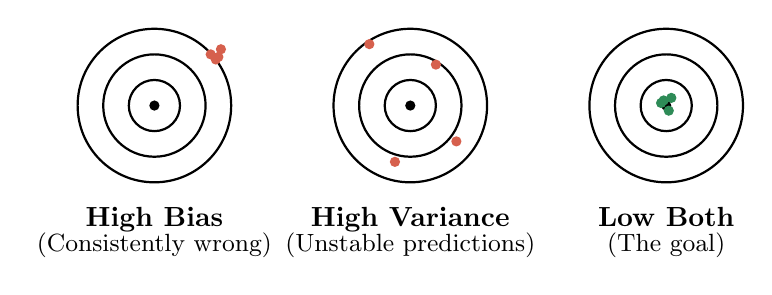
\begin{tikzpicture}[scale=0.65]
    % High Bias, Low Variance
    \draw[thick] (0,0) circle (1.5);
    \draw[thick] (0,0) circle (1);
    \draw[thick] (0,0) circle (0.5);
    \fill (0,0) circle (0.1);
    \foreach \x/\y in {1.2/0.9, 1.3/1.1, 1.1/1.0, 1.25/0.95} {
      \fill[AccentOrange] (\x,\y) circle (0.1);
    }
    \node[below] at (0,-1.8) {\textbf{High Bias}};
    \node[below] at (0,-2.3) {\small (Consistently wrong)};
    
    % Low Bias, High Variance
    \begin{scope}[xshift=5cm]
    \draw[thick] (0,0) circle (1.5);
    \draw[thick] (0,0) circle (1);
    \draw[thick] (0,0) circle (0.5);
    \fill (0,0) circle (0.1);
    \foreach \x/\y in {-0.8/1.2, 0.9/-0.7, -0.3/-1.1, 0.5/0.8} {
      \fill[AccentOrange] (\x,\y) circle (0.1);
    }
    \node[below] at (0,-1.8) {\textbf{High Variance}};
    \node[below] at (0,-2.3) {\small (Unstable predictions)};
    \end{scope}
    
    % Low Bias, Low Variance (ideal)
    \begin{scope}[xshift=10cm]
    \draw[thick] (0,0) circle (1.5);
    \draw[thick] (0,0) circle (1);
    \draw[thick] (0,0) circle (0.5);
    \fill (0,0) circle (0.1);
    \foreach \x/\y in {0.1/0.15, -0.1/0.05, 0.05/-0.1, -0.05/0.1} {
      \fill[AccentGreen] (\x,\y) circle (0.1);
    }
    \node[below] at (0,-1.8) {\textbf{Low Both}};
    \node[below] at (0,-2.3) {\small (The goal)};
    \end{scope}
  \end{tikzpicture}
  \end{center}
  
  \vspace{0.3em}
  \small
  \begin{itemize}
    \item Bullseye = true relationship $f(X)$ we are trying to learn
    \item Each dart = prediction from model trained on a different sample
    \item \textbf{Bias:} How far is the \emph{average} prediction from the truth?
    \item \textbf{Variance:} How much do predictions \emph{scatter} across samples?
  \end{itemize}
\end{frame}

\begin{frame}{Visual Example: Fitting a Curve}
  \begin{center}
  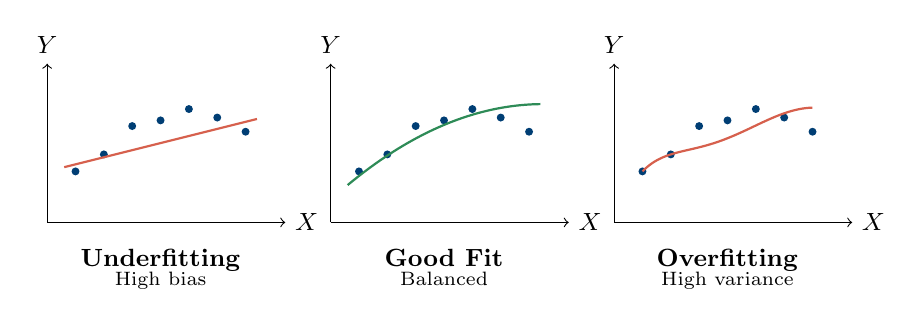
\begin{tikzpicture}[scale=0.72]
    % Data points coordinates
    \def\points{{0.5,0.9}, {1.0,1.2}, {1.5,1.7}, {2.0,1.8}, {2.5,2.0}, {3.0,1.85}, {3.5,1.6}}
    
    % Underfitting
    \begin{scope}
      \draw[->] (0,0) -- (4.2,0) node[right] {\small $X$};
      \draw[->] (0,0) -- (0,2.8) node[above] {\small $Y$};
      % Points
      \foreach \x/\y in {0.5/0.9, 1.0/1.2, 1.5/1.7, 2.0/1.8, 2.5/2.0, 3.0/1.85, 3.5/1.6} {
        \fill[ThemeBlue] (\x,\y) circle (0.07);
      }
      % Simple line (underfitting)
      \draw[thick, AccentOrange, domain=0.3:3.7] plot (\x, {0.9 + 0.25*\x});
      \node[below] at (2,-0.3) {\small \textbf{Underfitting}};
      \node[below] at (2,-0.7) {\scriptsize High bias};
    \end{scope}
    
    % Good fit
    \begin{scope}[xshift=5cm]
      \draw[->] (0,0) -- (4.2,0) node[right] {\small $X$};
      \draw[->] (0,0) -- (0,2.8) node[above] {\small $Y$};
      \foreach \x/\y in {0.5/0.9, 1.0/1.2, 1.5/1.7, 2.0/1.8, 2.5/2.0, 3.0/1.85, 3.5/1.6} {
        \fill[ThemeBlue] (\x,\y) circle (0.07);
      }
      % Smooth curve (good fit)
      \draw[thick, AccentGreen, domain=0.3:3.7, samples=50] 
        plot (\x, {0.4 + 0.9*\x - 0.12*\x*\x});
      \node[below] at (2,-0.3) {\small \textbf{Good Fit}};
      \node[below] at (2,-0.7) {\scriptsize Balanced};
    \end{scope}
    
    % Overfitting
    \begin{scope}[xshift=10cm]
      \draw[->] (0,0) -- (4.2,0) node[right] {\small $X$};
      \draw[->] (0,0) -- (0,2.8) node[above] {\small $Y$};
      \foreach \x/\y in {0.5/0.9, 1.0/1.2, 1.5/1.7, 2.0/1.8, 2.5/2.0, 3.0/1.85, 3.5/1.6} {
        \fill[ThemeBlue] (\x,\y) circle (0.07);
      }
      % Interpolating curve (overfitting) - passes through all points
      \draw[thick, AccentOrange, domain=0.5:3.5, samples=100] 
        plot (\x, {0.9 + 0.6*(\x-0.5) - 0.35*(\x-0.5)*(\x-1) + 0.28*(\x-0.5)*(\x-1)*(\x-1.5) - 0.12*(\x-0.5)*(\x-1)*(\x-1.5)*(\x-2) + 0.02*(\x-0.5)*(\x-1)*(\x-1.5)*(\x-2)*(\x-2.5)});
      \node[below] at (2,-0.3) {\small \textbf{Overfitting}};
      \node[below] at (2,-0.7) {\scriptsize High variance};
    \end{scope}
  \end{tikzpicture}
  \end{center}
  
  \vspace{0.5em}
  \begin{itemize}
    \item \textbf{Left:} Straight line misses the curvature in the data
    \item \textbf{Middle:} Smooth curve captures the overall pattern
    \item \textbf{Right:} Wiggly curve passes through every point --- but will fail on new data
  \end{itemize}
\end{frame}

\begin{frame}{The Bias-Variance Decomposition}
  \textbf{Mathematical fact:} The expected test error decomposes into three parts
  \[
  \underbrace{\mathbb{E}\left[(Y - \widehat{f}(X))^2\right]}_{\text{What we care about}} = \underbrace{\text{Bias}^2}_{\text{How Wrong is $\widehat{f}$}} + \underbrace{\text{Variance}}_{\text{How Unstable is $\widehat{f}$}} + \underbrace{\sigma^2}_{\text{Irreducible noise}}
  \]
  
  \vspace{0.5em}
  \begin{itemize}
    \item $\sigma^2$ is the inherent unpredictability --- even the best model can't eliminate it
    \item We control Bias and Variance through model choice
    \item \highlight{Minimizing test error requires balancing Bias and Variance}
  \end{itemize}
  
  \vspace{0.5em}
  \begin{center}
    \begin{tabular}{lcc}
    \toprule
    & \textbf{Simple Model} & \textbf{Complex Model} \\
    \midrule
    Bias & High & Low \\
    Variance & Low & High \\
    \bottomrule
    \end{tabular}
  \end{center}
\end{frame}




\begin{frame}{Complexity vs. Error: The Classic Picture}
  \begin{center}
  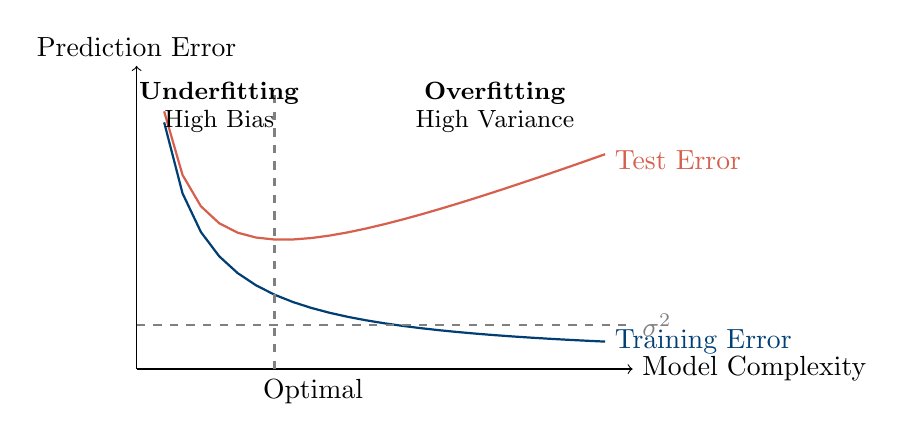
\begin{tikzpicture}[scale=0.7]
    % Axes
    \draw[->] (0,0) -- (9,0) node[right] {Model Complexity};
    \draw[->] (0,0) -- (0,5.5) node[above] {Prediction Error};
    
    % Training error (always decreasing)
    \draw[thick, ThemeBlue, domain=0.5:8.5] 
      plot (\x, {3.5/(\x+0.3) + 0.1});
    \node[ThemeBlue, right] at (8.5, 0.5) {Training Error};
    
    % Test error (U-shaped)
    \draw[thick, AccentOrange, domain=0.5:8.5] 
      plot (\x, {3.5/(\x+0.3) + 0.4*(\x-0.5) + 0.3});
    \node[AccentOrange, right] at (8.5, 3.8) {Test Error};
    
    % Optimal point
    \draw[thick, dashed, gray] (2.5,0) -- (2.5,5);
    \node[below] at (3.2,0) {Optimal};
    
    % Regions
    \node at (1.5, 5) {\small \textbf{Underfitting}};
    \node at (1.5, 4.5) {\small High Bias};
    \node at (6.5, 5) {\small \textbf{Overfitting}};
    \node at (6.5, 4.5) {\small High Variance};
    
    % Irreducible error
    \draw[thick, dashed, gray] (0,0.8) -- (9,0.8);
    \node[gray, right] at (9, 0.8) {$\sigma^2$};
  \end{tikzpicture}
  \end{center}
  
  \textbf{Key observation:}
  \begin{itemize}
    \item Training error always decreases with complexity
    \item Test error has a U-shape --- there's a sweet spot
    \item \highlight{We must estimate test error to choose optimal complexity}
  \end{itemize}
\end{frame}

\begin{frame}{Why Overfitting Is Deadly in Finance}
  \textbf{Finance is especially prone to overfitting because:}
  \begin{itemize}
    \item Signal-to-noise ratio is very low (markets are near-efficient)
    \item Many candidate predictors (300+ characteristics documented)
    \item Limited independent observations (monthly data = 12 per year)
    \item Predictive relationships may change over time (regime shifts)
  \end{itemize}
  
  \vspace{0.5em}
  \textbf{The evidence (Harvey, Liu \& Zhu, 2016):}
  \begin{itemize}
    \item Surveyed 300+ factors published in top finance journals
    \item Most factors that ``worked'' in-sample do not replicate
    \item Key culprit: researchers test many strategies, publish only winners
  \end{itemize}
  
  \vspace{0.5em}
  \begin{block}{Mantra}
    If it seems too good to be true, it is probably overfitting
  \end{block}
\end{frame}

%----------------------------------------------------------------------------------------
\section{Model Validation: Estimating Test Error}
%----------------------------------------------------------------------------------------

\begin{frame}{The Validation Problem}
  \textbf{We need to estimate test error, but we only have training data!}
  
  \vspace{0.5em}
  \textbf{Naive approach:} Use training error
  \begin{itemize}
    \item Problem: Training error is too optimistic (see previous discussion)
    \item Complex models can achieve zero training error while being useless
  \end{itemize}
  
  \vspace{0.5em}
  \textbf{Solution:} Hold out some data for validation
  \begin{itemize}
    \item Don't use it for training
    \item Use it to estimate how well we would do on new data
  \end{itemize}
  
  \vspace{0.5em}
  \begin{block}{General Principle}
    The data you use to evaluate a model must be different from the data you used to build it
  \end{block}
\end{frame}

\begin{frame}{Train-Validation-Test Split}
  \textbf{Standard approach:} Divide your data into three parts
  
  \vspace{0.5em}
  \begin{center}
  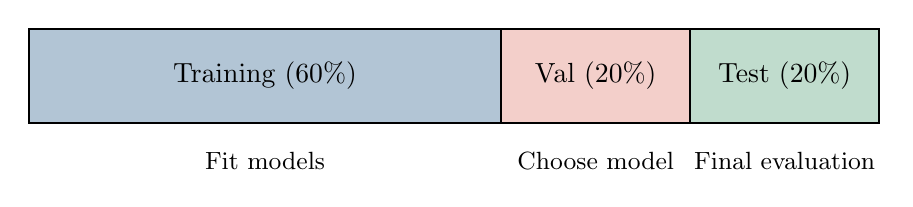
\begin{tikzpicture}[scale=1.2]
    \draw[thick, fill=ThemeBlue!30] (0,0) rectangle (5,1);
    \draw[thick, fill=AccentOrange!30] (5,0) rectangle (7,1);
    \draw[thick, fill=AccentGreen!30] (7,0) rectangle (9,1);
    
    \node at (2.5, 0.5) {Training (60\%)};
    \node at (6, 0.5) {Val (20\%)};
    \node at (8, 0.5) {Test (20\%)};
    
    \node[below, align=center] at (2.5, -0.2) {\small Fit models};
    \node[below, align=center] at (6, -0.2) {\small Choose model};
    \node[below, align=center] at (8, -0.2) {\small Final evaluation};
  \end{tikzpicture}
  \end{center}
  
  \vspace{0.5em}
  \begin{enumerate}
    \item \textbf{Training set:} Fit different models
    \item \textbf{Validation set:} Compare models, choose the best one 
    \item \textbf{Test set:} Evaluate final model (touch only once!)
  \end{enumerate}
  
  \vspace{1em}
  \textbf{Why three sets?}
  \begin{itemize}
    \item Validation set gets ``used up'' as we try different models
    \item Test set gives honest final assessment
  \end{itemize}
\end{frame}

\begin{frame}{Cross-Validation: Using Data More Efficiently}
  \textbf{Problem:} Holding out 40\% of data reduces training sample
  
  \vspace{0.5em}
  \textbf{Solution:} \highlight{K-Fold Cross-Validation}
  
  \begin{center}
  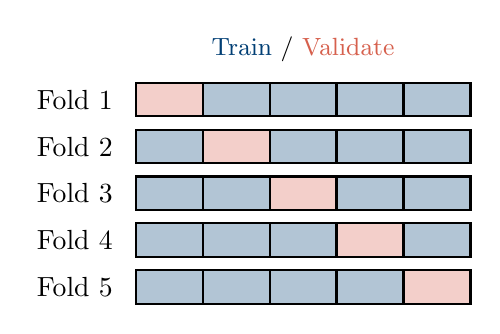
\begin{tikzpicture}[scale=0.85]
    \foreach \i in {1,...,5} {
      \foreach \j in {1,...,5} {
        \ifnum\j=\i
          \draw[thick, fill=AccentOrange!30] (\j-1, -\i*0.7) rectangle (\j, -\i*0.7+0.5);
        \else
          \draw[thick, fill=ThemeBlue!30] (\j-1, -\i*0.7) rectangle (\j, -\i*0.7+0.5);
        \fi
      }
      \node[left] at (-0.2, -\i*0.7+0.25) {Fold \i};
    }
    \node at (2.5, 0.3) {\small \textcolor{ThemeBlue}{Train} / \textcolor{AccentOrange}{Validate}};
  \end{tikzpicture}
  \end{center}
  
  \textbf{Procedure:}
  \begin{enumerate}
    \item Split data into K equal parts (``folds'')
    \item For each fold: train on other K-1 folds, validate on this fold
    \item Average the K validation errors
  \end{enumerate}
  
  \textbf{Common choice:} K = 5 or K = 10
\end{frame}

\begin{frame}{Problem: Random CV Doesn't Work for Time Series!}
  \textbf{Financial data is ordered in time.} Random splits cause problems:
  
  \vspace{0.5em}
  \begin{center}
  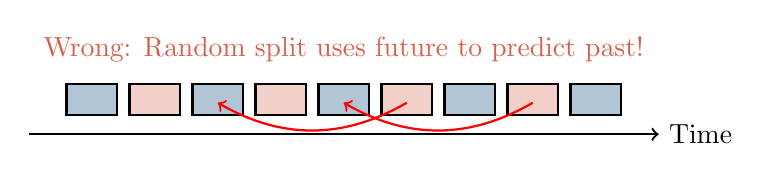
\begin{tikzpicture}[scale=0.8]
    \draw[thick, ->] (0,0) -- (10,0) node[right] {Time};
    
    % Wrong way
    \foreach \x in {1,3,5,7,9} {
      \draw[thick, fill=ThemeBlue!30] (\x-0.4, 0.3) rectangle (\x+0.4, 0.8);
    }
    \foreach \x in {2,4,6,8} {
      \draw[thick, fill=AccentOrange!30] (\x-0.4, 0.3) rectangle (\x+0.4, 0.8);
    }
    
    \node[above] at (5, 1) {\bad{Wrong: Random split uses future to predict past!}};
    
    % Arrows showing problem
    \draw[->, thick, red] (6, 0.5) to[bend left] (3, 0.5);
    \draw[->, thick, red] (8, 0.5) to[bend left] (5, 0.5);
  \end{tikzpicture}
  \end{center}
  
  \vspace{0.5em}
  \textbf{This creates \highlight{look-ahead bias}:}
  \begin{itemize}
    \item Training on 2020 data to ``predict'' 2018 returns
    \item Model learns from information that would not exist at prediction time
    \item Overly optimistic performance estimates
  \end{itemize}
\end{frame}

\begin{frame}{Time-Series Cross-Validation}
  \textbf{Solution:} Only use past data to predict future data (Walk-Forward Validation)
  
  \vspace{0.5em}
  \begin{center}
  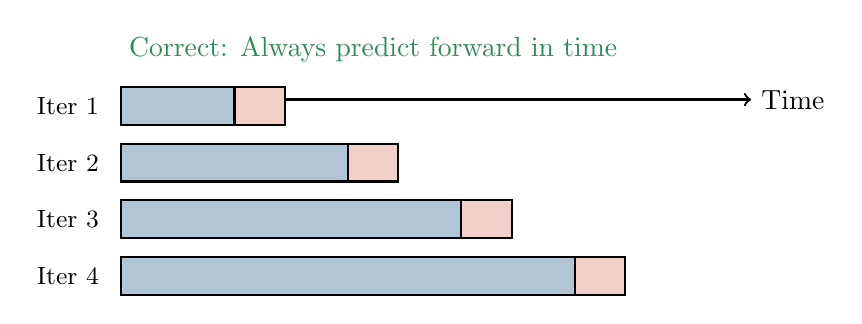
\begin{tikzpicture}[scale=0.8]
    \draw[thick, ->] (0,-0.5) -- (10,-0.5) node[right] {Time};
    
    \foreach \i in {1,...,4} {
      % Training period
      \draw[thick, fill=ThemeBlue!30] (0,-\i*0.9) rectangle (\i*1.8, -\i*0.9+0.6);
      % Validation period  
      \draw[thick, fill=AccentOrange!30] (\i*1.8,-\i*0.9) rectangle (\i*1.8+0.8, -\i*0.9+0.6);
      \node[left] at (-0.2, -\i*0.9+0.3) {\small Iter \i};
    }
    
    \node at (4, 0.3) {\good{Correct: Always predict forward in time}};
  \end{tikzpicture}
  \end{center}
  
  \vspace{0.3em}
  \textbf{Two variants:}
  \begin{itemize}
    \item \textbf{Expanding window:} Use all past data (shown above)
    \item \textbf{Rolling window:} Fixed-size training window (discards old data)
  \end{itemize}
\end{frame}


\begin{frame}{The Golden Rule of Out-of-Sample Testing}
  \begin{block}{The Rule}
    \centering
    Once you look at test set results, the test set is contaminated.\\
    You get \textbf{one shot} at honest out-of-sample evaluation.
  \end{block}
  
  \vspace{0.5em}
  \textbf{Why?}
  \begin{itemize}
    \item If you adjust model selection/estimation based on test results, you are implicitly fitting to the test set
    \item This is exactly the overfitting problem we are trying to avoid
    \item Performance will be overestimated in a realistic setting
  \end{itemize}
  
  \vspace{0.5em}
  \textbf{Best practice:}
  \begin{enumerate}
    \item Do all model selection on training + validation data
    \item Lock in your final model choice
    \item Only then evaluate on test set
    \item Report the test result, \highlight{even if disappointing}
  \end{enumerate}
\end{frame}

%======================== PART II CONTENT ========================

\section{Common Pitfalls in Financial Machine Learning}
%----------------------------------------------------------------------------------------

\begin{frame}{Why Financial ML Is Especially Hard}
  \textbf{Recall from previous slides:} Overfitting is deadly in finance.
  
  \vspace{1em}
  \textbf{Three additional pitfalls specific to financial applications:}
  
  \vspace{0.5em}
  \begin{enumerate}
    \item \highlight{Look-ahead bias} — Using information you would not have at prediction time
    \vspace{0.3em}
    \item \highlight{Survivorship bias} — Only analyzing firms/funds that survived
    \vspace{0.3em}
    \item \highlight{Data snooping} — Testing many strategies, reporting only winners
  \end{enumerate}
  
  \vspace{1em}
  Each of these makes backtested performance look better than reality.
  
  \vspace{0.5em}
  \begin{block}{Key Insight}
    A strategy can fail for reasons beyond overfitting — even a properly validated model can \emph{``be garbage in, garbage out.''}
  \end{block}
\end{frame}

\begin{frame}{Look-Ahead Bias}
  \textbf{Definition:} Using information that would not have been available at the time the prediction was made.
  
  \vspace{1em}
  \textbf{Common sources:}
  \begin{itemize}
    \item \highlight{Timing of data releases:} Using Q4 earnings announced in February to ``predict'' January returns
    \item \highlight{Restated financials:} Using corrected accounting data, not original reports
    \item \highlight{Point-in-time vs. revised data:} Economic indicators (e.g., GDP, Inflation, Unemployment) are often revised months later
    \item \highlight{Index membership:} Using current S\&P 500 constituents for a 1990 backtest
  \end{itemize}
  
  \vspace{1em}
  \textbf{Example:}
  \begin{itemize}
    \item You build a model using book value reported in Compustat
    \item But Compustat shows the \emph{final} value, not what was known at the first-time release
    \item Your model ``knows'' things investors could not have known
  \end{itemize}
\end{frame}

\begin{frame}{Look-Ahead Bias: How to Avoid It}
  \textbf{Best practices:}
  
  \vspace{0.5em}
  \begin{enumerate}
    \item \textbf{Use point-in-time databases} when available
    \begin{itemize}
      \item CRSP, Compustat with proper date alignment
      \item IBES for analyst forecasts with announcement dates
    \end{itemize}
    \vspace{0.3em}
    \item \textbf{Apply realistic lags}
    \begin{itemize}
      \item Quarterly data: available $\approx$45 days after quarter end
      \item Annual data: available $\approx$90 days after fiscal year end
    \end{itemize}
    \vspace{0.3em}
    \item \textbf{Be explicit about timing}
    \begin{itemize}
      \item Document when each feature was knowable/observable
      \item Build this into your data pipeline
    \end{itemize}
    \vspace{0.3em}
    \item \textbf{Use walk-forward validation} (as discussed in previous slides)
  \end{enumerate}
  
  \vspace{0.5em}
  \begin{block}{Rule of Thumb}
    When in doubt, add one (or more) lag(s). Being conservative hurts less than look-ahead bias.
  \end{block}
\end{frame}

\begin{frame}{Survivorship Bias}
  \textbf{Definition:} Analyzing only entities that ``survived'' to the present, ignoring those that failed, delisted, or disappeared.
  
  \vspace{1em}
  \highlight{Why it matters:}
  \begin{itemize}
    \item Failed companies often had distinct characteristics before failure
    \item Excluding them biases your sample toward ``winners''
    \item Relationships estimated on survivors may not hold in the full population, which also includes the ``losers''
  \end{itemize}
  
  \vspace{1em}
  \textbf{Classic examples:}
  \begin{itemize}
    \item \textbf{Mutual funds:} Databases often drop funds that close; remaining funds look better on average
    \item \textbf{Hedge funds:} Voluntary reporting + fund closures = severe upward bias
    \item \textbf{Stocks:} Using only current exchange members misses delistings
  \end{itemize}

\end{frame}

\begin{frame}{Survivorship Bias: How to Avoid It}
  \textbf{Best practices:}
  
  \vspace{0.5em}
  \begin{enumerate}
    \item \textbf{Use survivorship-bias-free databases}
    \begin{itemize}
      \item CRSP includes delisted stocks with delisting returns
      \item Check if your data source retains ``dead'' entities
    \end{itemize}
    \vspace{0.3em}
    \item \textbf{Include delisting returns}
    \begin{itemize}
      \item When a stock delists, there is often a final return (often negative)
      \item Ignoring this overstates strategy performance
    \end{itemize}
    \vspace{0.3em}
    \item \textbf{Be skeptical of ``cleaned'' datasets}
    \begin{itemize}
      \item Sometimes cleaning removes exactly the observations you need
      \item Understand what was removed and why
    \end{itemize}
    \vspace{0.3em}
    \item \textbf{For credit risk:} Ensure you include loans/mortgages that defaulted, not just those that were fully or partly repaid
  \end{enumerate}
\end{frame}

\begin{frame}{Data Snooping and Multiple Testing}
  \textbf{Definition:} Testing many hypotheses/strategies on the same data and selectively reporting the winners.
  
  \vspace{1em}
  \textbf{The problem:}
  \begin{itemize}
    \item With 100 random strategies, $\sim$5 will appear significant at the 5\% level by chance
    \item If you only report the winners, they look real
    \item This happens implicitly through researcher degrees of freedom
  \end{itemize}
  
  \vspace{1em}
  \textbf{Forms of data snooping:}
  \begin{itemize}
    \item Trying many feature combinations, keeping what works
    \item Testing multiple model specifications
    \item Optimizing hyperparameters on the same data used for evaluation
    \item ``Peeking'' at test data to guide model development
  \end{itemize}
  
  \vspace{0.5em}
  \textbf{Harvey, Liu \& Zhu (2016):} Many published factors are likely false discoveries due to collective data snooping across the literature.
\end{frame}

\begin{frame}{Data Snooping: How to Mitigate It}
  \textbf{No perfect solution, but several defenses:}
  
  \vspace{0.5em}
  \begin{enumerate}
    \item \textbf{Adjust for multiple testing}
    \begin{itemize}
      \item Bonferroni correction: divide significance level by number of tests
      \item More sophisticated: Benjamini-Hochberg for false discovery rate
      \item \textbf{Chordia, Goyal, and Saretto (2020):} you need to adjust for portfolio return correlations. 
    \end{itemize}
    \vspace{0.3em}
    \item \textbf{Pre-registration}
    \begin{itemize}
      \item Commit to methodology before seeing results
      \item Common in medicine, emerging in finance
    \end{itemize}
    \vspace{0.3em}
    \item \textbf{True out-of-sample testing}
    \begin{itemize}
      \item Hold out data you genuinely never look at
      \item Or use new data that arrives after model development
    \end{itemize}
    \vspace{0.3em}
    \item \textbf{Economic plausibility}
    \begin{itemize}
      \item Does the pattern make sense? Is there a ``story'' to be told?
      \item Pure statistical patterns without economic rationale are suspect
    \end{itemize}
  \end{enumerate}
\end{frame}

\begin{frame}{Summary: A Checklist for Honest Backtests}
  Before trusting any ML strategy in finance, verify:
  
  \vspace{0.5em}
  \begin{enumerate}
    \item[\checkmark] \textbf{No look-ahead bias}
    \begin{itemize}
      \item All features use only information available at prediction time
    \end{itemize}
    \vspace{0.3em}
    \item[\checkmark] \textbf{No survivorship bias}
    \begin{itemize}
      \item Sample includes failed/delisted entities
    \end{itemize}
    \vspace{0.3em}
    \item[\checkmark] \textbf{Proper validation}
    \begin{itemize}
      \item Time-series CV, not random splits
      \item Clean separation of train/validation/test
    \end{itemize}
    \vspace{0.3em}
    \item[\checkmark] \textbf{Multiple testing adjustment}
    \begin{itemize}
      \item Account for all strategies tried, not just the winner
    \end{itemize}
    \vspace{0.3em}
    \item[\checkmark] \textbf{Economic sensibility}
    \begin{itemize}
      \item Results have plausible interpretation
    \end{itemize}
  \end{enumerate}
  
  \vspace{0.5em}
  \highlight{If a study does not address these, treat results with skepticism.}
\end{frame}

%----------------------------------------------------------------------------------------
\section{Python for Machine Learning}
%----------------------------------------------------------------------------------------

\begin{frame}{Why Python?}
  \textbf{Python has become the dominant language for ML in finance:}
  
  \vspace{0.5em}
  \begin{itemize}
    \item Rich ecosystem of ML libraries
    \item Strong data manipulation tools
    \item Good integration with databases and APIs
    \item Large community and documentation
    \item Used by major quant firms and fintech companies
  \end{itemize}
  
  \vspace{1em}
  \textbf{Alternatives:}
  \begin{itemize}
    \item \textbf{R:} Strong for statistics, less so for production deployment
    \item \textbf{Julia:} Fast, but smaller ecosystem
    \item \textbf{MATLAB:} Common in academia, expensive, less ML support
  \end{itemize}
  
  \vspace{0.5em}
  \textbf{This course:} All implementation in Python using industry-standard libraries
\end{frame}

\begin{frame}{Core Libraries We Will Use}
  \begin{center}
  \begin{tabular}{lll}
    \toprule
    \textbf{Library} & \textbf{Purpose} & \textbf{Key Use} \\
    \midrule
    \texttt{numpy} & Numerical computing & Arrays, linear algebra \\
    \texttt{pandas} & Data manipulation & DataFrames, time series \\
    \texttt{scikit-learn} & Machine learning & Models, pipelines, CV \\
    \texttt{matplotlib} & Visualization & Basic plots \\
    \texttt{seaborn} & Visualization & Statistical graphics \\
    \midrule
    \texttt{xgboost} & Gradient boosting & Tree ensembles \\
    \texttt{lightgbm} & Gradient boosting & Fast tree ensembles \\
    \texttt{shap} & Interpretability & Model explanations \\
    \bottomrule
  \end{tabular}
  \end{center}
  
  \vspace{1em}
  \textbf{Focus:} We use \texttt{scikit-learn} as our primary ML library.
  \begin{itemize}
    \item Consistent API across all models
    \item Built-in cross-validation and pipelines
    \item Good documentation and examples
  \end{itemize}
\end{frame}

\begin{frame}[fragile]{The Scikit-Learn API Pattern}
  \textbf{All scikit-learn models follow the same pattern:}
  
  \vspace{0.5em}
\begin{verbatim}
    from sklearn.linear_model import Ridge
    
    # 1. Create model with hyperparameters
    model = Ridge(alpha=1.0)
    
    # 2. Fit to training data
    model.fit(X_train, y_train)
    
    # 3. Make predictions
    predictions = model.predict(X_test)
    
    # 4. Evaluate
    score = model.score(X_test, y_test)
\end{verbatim}
  
  \vspace{0.5em}
  \highlight{This works for any model:} \texttt{Lasso}, \texttt{RandomForestRegressor}, etc.
  
  \vspace{0.5em}
  Once you learn this pattern, switching between models is trivial.
\end{frame}

\begin{frame}[fragile]{Pipelines: Combining Steps}
  \textbf{Real ML workflows have multiple steps:} (1) Handle missing values and outliers, (2) Scale features and pre-processing, and (3) Fit model
    
  \vspace{1em}
  \textbf{Pipelines bundle these together:}
  
\begin{verbatim}
    from sklearn.pipeline import Pipeline
    from sklearn.preprocessing import StandardScaler
    from sklearn.impute import SimpleImputer
    
    pipeline = Pipeline([
        ('imputer', SimpleImputer(strategy='median')),
        ('scaler', StandardScaler()),
        ('model', Ridge(alpha=1.0))
    ])
    
    pipeline.fit(X_train, y_train)
    predictions = pipeline.predict(X_test)
\end{verbatim}
  
  \vspace{0.3em}
  \textbf{Benefits:} Prevents data leakage, easy to save/deploy, cleaner code
\end{frame}

\begin{frame}[fragile]{Time-Series CV in Scikit-Learn}
  \textbf{Scikit-learn provides \texttt{TimeSeriesSplit}:}
  
  \vspace{0.5em}
\begin{verbatim}
    from sklearn.model_selection import TimeSeriesSplit
    from sklearn.model_selection import cross_val_score
    
    # Create time-series splitter
    tscv = TimeSeriesSplit(n_splits=5)
    
    # Cross-validate respecting time order
    scores = cross_val_score(model, X, y, cv=tscv)
    
    print(f"Mean CV Score: {scores.mean():.4f}")
\end{verbatim}
  
  \vspace{0.5em}
  \highlight{Implementing the walk-forward validation from previous slides becomes trivial in Python.}
  
  \vspace{0.5em}
  \textbf{Note:} Data must be sorted by time before using \texttt{TimeSeriesSplit}!
\end{frame}


%----------------------------------------------------------------------------------------
\section{A Bird's Eye View on Empirical Applications}
%----------------------------------------------------------------------------------------

\begin{frame}{Two Running Applications}
  \textbf{Throughout this course, we apply ML methods to two problems:}
  
  \vspace{1em}
  \begin{columns}[T]
    \column{0.48\textwidth}
    \textbf{1. Market Timing}
    \begin{itemize}
      \item Forecast the aggregate stock market return over time
      \item A \emph{time-series} problem: when is the market expected to do well or poorly?
      \item Use macroeconomic and valuation predictors to time the market
      \item Lectures 2, 3, 4, 7, 9
    \end{itemize}
    
    \column{0.48\textwidth}
    \textbf{2. Credit Risk}
    \begin{itemize}
      \item Predict loan/mortgage defaults
      \item Classification problem
      \item Handle class imbalance
      \item Build credit scorecards and implement credit assessment and monitoring tools
      \item Lectures 5, 6, 8
    \end{itemize}
  \end{columns}
  
  \vspace{1em}
  \textbf{Why these two?}
  \begin{itemize}
    \item Cover regression and classification
    \item Represent major industry applications
    \item Rich datasets available
  \end{itemize}
\end{frame}

\begin{frame}{Application 1: Market Timing}
  \textbf{The setup:}
  \begin{itemize}
    \item Target: next month's aggregate market excess return, $r_{m,t+1}$
    \item Predictors: macroeconomic and valuation variables known at time $t$
    \item A \emph{time-series} forecasting problem
  \end{itemize}

  \vspace{0.5em}
  \textbf{Typical predictors (15--20 from the literature):}
  \begin{itemize}
    \item \textbf{Valuation ratios:} dividend-price, earnings-price, book-to-market
    \item \textbf{Interest rates:} T-bill rate, term spread, default spread
    \item \textbf{Other:} stock variance, inflation, net equity expansion
  \end{itemize}

  \vspace{0.5em}
  \textbf{Key questions we will address:}
  \begin{itemize}
    \item Can we beat the historical mean out-of-sample?
    \item Is there genuine economic value in timing the market?
    \item Do ML methods help, or do they just overfit?
  \end{itemize}
\end{frame}

\begin{frame}{Application 1: From Forecasts to Allocations}
  \textbf{A return forecast is only useful if it improves decisions.}

  \vspace{1em}
  \textbf{Typical workflow:}
  \begin{enumerate}
    \item Forecast next month's market return $\widehat{r}_{m,t+1}$
    \item Translate the forecast into an equity allocation (e.g., shift between stocks and bonds)
    \item Rebalance as new information arrives
    \item Measure performance against a buy-and-hold benchmark
  \end{enumerate}

  \vspace{0.5em}
  \textbf{Performance metrics:}
  \begin{itemize}
    \item Out-of-sample $R^2$ vs.\ the historical mean (often tiny --- even $\sim$0.5\% per month is economically meaningful)
    \item Sharpe ratio of the timing strategy
    \item Certainty-equivalent / utility gains for a mean-variance investor
    \item Turnover and transaction costs
  \end{itemize}

  \vspace{0.5em}
  \textbf{Spoiler:} Generating genuine out-of-sample economic value (net of transaction costs) is more difficult than you would think.
\end{frame}

\begin{frame}{Application 2: Credit Risk}
  \textbf{The setup:}
  \begin{itemize}
    \item Data: LendingClub peer-to-peer loans
    \item Features: Borrower characteristics, loan terms
    \item Target: Default (yes/no) — a \emph{classification} problem
  \end{itemize}
  
  \vspace{0.5em}
  \textbf{Types of features:}
  \begin{itemize}
    \item \textbf{Borrower:} Income, employment length, home ownership
    \item \textbf{Credit history:} FICO score, delinquencies, credit utilization
    \item \textbf{Loan:} Amount, interest rate, purpose, term
  \end{itemize}
  
  \vspace{0.5em}
  \textbf{Key challenges:}
  \begin{itemize}
    \item \textbf{Class imbalance:} Defaults are rare ($\sim$10--20\%)
    \item \textbf{Probability calibration:} Need accurate default probabilities
    \item \textbf{Interpretability:} Regulators require explanations
    \item \textbf{Fairness:} Cannot discriminate on protected characteristics
  \end{itemize}
\end{frame}

\begin{frame}{Application 2: From Predictions to Decisions}
  \textbf{Credit predictions feed into business decisions:}
  
  \vspace{1em}
  \textbf{Use cases:}
  \begin{enumerate}
    \item \textbf{Approve/reject:} Set threshold on predicted default probability
    \item \textbf{Pricing:} Charge higher interest to riskier borrowers
    \item \textbf{Portfolio management:} Allocate capital across risk buckets
    \item \textbf{Regulatory capital:} Calculate required reserves
  \end{enumerate}
  
  \vspace{0.5em}
  \textbf{Performance metrics:}
  \begin{itemize}
    \item AUC-ROC (ranking quality)
    \item Precision/Recall at decision threshold
    \item Expected loss vs. actual loss
    \item Calibration: Do 10\% predicted defaults actually default 10\%?
  \end{itemize}
  
  \vspace{0.5em}
  \textbf{Reference:} Khandani, Kim \& Lo (2010) show ML methods significantly outperform traditional credit scorecards.
\end{frame}


%----------------------------------------------------------------------------------------
\section{Summary and Next Steps}
%----------------------------------------------------------------------------------------


\begin{frame}{Key Takeaways from Lecture 1}
  \begin{enumerate}
    \item ML focuses on prediction; we learn $\widehat{f}$ from data
    \item Bias-variance tradeoff governs model selection
    \item Time-series CV is essential for financial applications
    \item Beware of look-ahead bias, survivorship bias, and data snooping
    \item Python + scikit-learn provide a consistent ML workflow
    \item We will apply methods to market timing and credit risk
  \end{enumerate}

  \vspace{1em}
  \begin{block}{The Bottom Line}
    ML offers powerful tools, but finance demands extra caution. A disciplined and rigorous approach to validation is essential.
  \end{block}
\end{frame}

\begin{frame}{Readings and Next Steps}
  \textbf{Readings for Today's Lecture:}
  \begin{itemize}
    \item James et al. (2023), \textit{An Introduction to Statistical Learning}, Chapters 2 and 5
    \item Harvey, Liu \& Zhu (2016), ``\ldots and the Cross-Section of Expected Returns,'' \textit{Review of Financial Studies}
    \item Gu, Kelly \& Xiu (2020), ``Empirical Asset Pricing via Machine Learning,'' \textit{Review of Financial Studies} (Introduction and Section 2)
    \item Chordia, Goyal \& Saretto (2020), ``Anomalies and False Rejections,'' \textit{Review of Financial Studies}
  \end{itemize}
  \vspace{1em}

  \textbf{Week 2 topics:}
  \begin{itemize}
    \item OLS limitations in high dimensions
    \item Ridge regression (L2 penalty)
    \item Lasso (L1 penalty, sparsity)
    \item Elastic Net (combining L1 and L2)
    \item Application: Market Timing and Factor Investing
  \end{itemize}
  
  

\end{frame}


\begin{frame}[plain]
  \centering
  \vfill
  {\Large Questions?}
  \vfill
\end{frame}


\end{document}